\section{Experimental details}\label{sec:appendix_experimental_details}

\subsection{Relational Games (\Cref{ssec:relgames})}\label{ssec:appendxi_relgames}

\begin{figure}
    \centering
    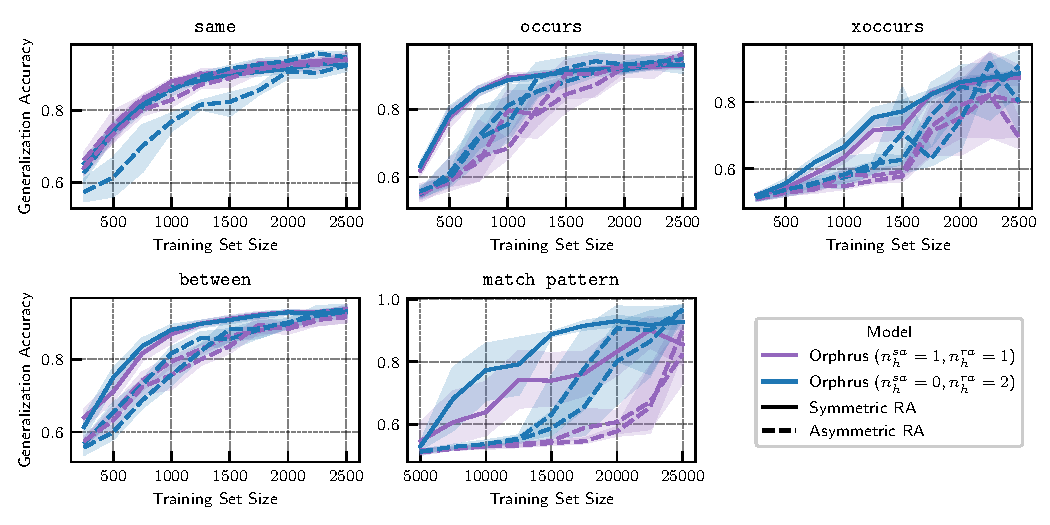
\includegraphics[width=\textwidth]{figs/experiments/relgames/relgames_learning_curves_symmetry_ablation.pdf}
    \caption{Ablation on effect of symmetry in relational attention.}
\end{figure}

\subsection{Mathematical Problem-Solving (\Cref{ssec:math})}\label{ssec:appendix_math}

\begin{figure}
    \centering
    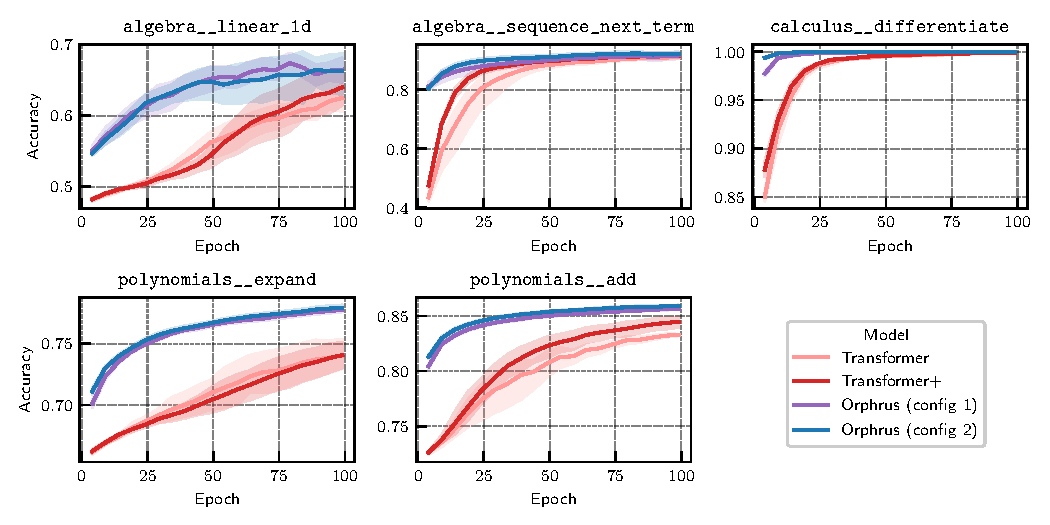
\includegraphics[width=\textwidth]{figs/experiments/math/math_training_curves_extrapolation.pdf}
    \caption{extrapolation accuracy curve}
\end{figure}

\begin{figure}
    \centering
    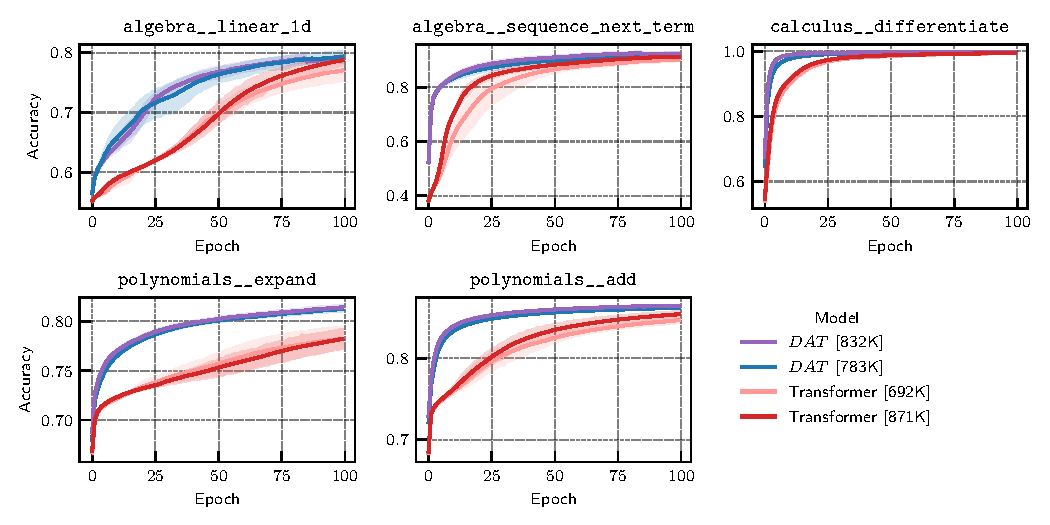
\includegraphics[width=\textwidth]{figs/experiments/math/math_training_curves_trainacc.pdf}
    \caption{Training accuracy curve}
\end{figure}
\aanote{need this? (math training acc curve)}


\subsection{Language Modeling (\Cref{ssec:tiny_stories})}\label{ssec:appendix_lm}

\begin{figure}
    \centering
    \begin{subfigure}{0.45\textwidth}
        \centering
        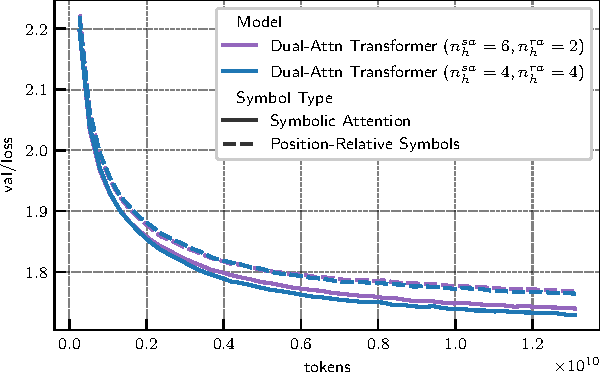
\includegraphics[width=\textwidth]{figs/experiments/tiny_stories/d64L4_ablation_symboltype_asymra.pdf}
        \caption{$d=64, L=4$, asymmetric RA}
    \end{subfigure}
    \begin{subfigure}{0.45\textwidth}
        \centering
        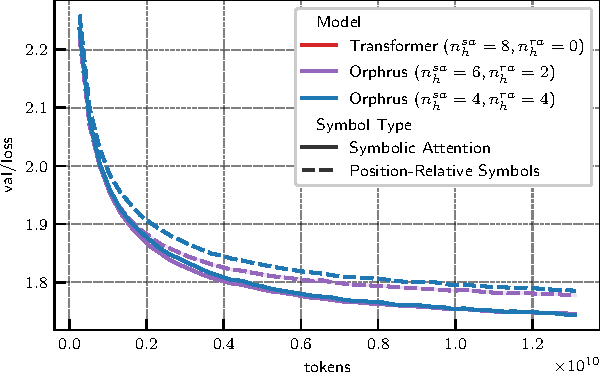
\includegraphics[width=\textwidth]{figs/experiments/tiny_stories/d64L4_ablation_symboltype_symra.pdf}
        \caption{$d=64, L=4$, symmetric RA}
    \end{subfigure}
    \caption{Ablation of symbol type}
\end{figure}

\begin{figure}
    \centering
    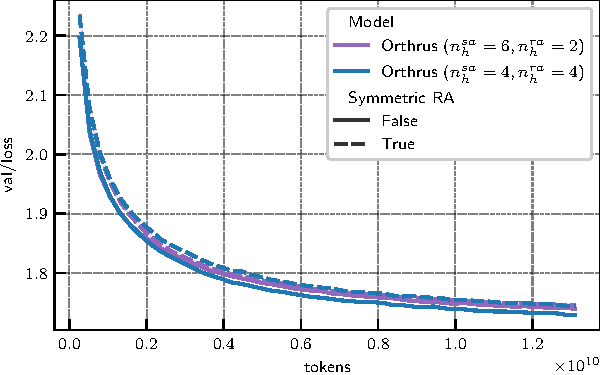
\includegraphics[width=0.5\textwidth]{figs/experiments/tiny_stories/d64L4_ablation_symmetry_symmattn.pdf}
    \caption{Ablation of symbol type}
\end{figure}

% add figure with d=128, L=4, 6